\chapter{Results and Evaluation}
\label{ch:evaluation}

This section will show a summary of of results, the raw results can be found in Appendix \ref{ch:raw-results}. 

Results are classified into True Positives ($TP$, declared real when real), True Negatives ($TN$, declared fake when fake), False Positives ($FP$, declared real when fake), and False Negatives ($FN$, declared fake when real). Overall accuracy is defined in Equation \ref{eq:acc} and accuracy on fake videos is defined by Equation \ref{eq:fake-acc}.

\begin{align}
    \text{Accuracy} &= \frac{TP+TN}{TP+TN+FP+FN} \label{eq:acc} \\
    \text{Fake Accuracy} &= \frac{TN}{TN+FP} \label{eq:fake-acc}
\end{align}

Traditional DeepFake detection uses the Area Under Curve (AUC) metric for model evaluation, which involves comparing the true positive rate against the false positive rate over all possible classification thresholds. AUC was not chosen for this project due to its tendency to over-inflate model performance by averaging results over a range of thresholds, most of which would be unsuitable for real-world implementations\cite{ricker2022towards}. Furthermore, in real-world applications, DeepFake detectors would operate at predetermined fixed thresholds which adversarial attacks would be fine-tuned to work against, hence an accuracy metric which varies such a threshold would be masking the true accuracy (or lack thereof) for a model.

\section{Proof of Concept}
\label{sec:concept-results}

% \begin{itemize}
%     \item initial results good
%     \item VGG19 was targeted and had was reduced to 0\% accuracy
%     \item ResNet however was not impacted
%     \item therefore noise is effective for the model it attacks
%     \item however other models not affected, need to test further
%     \item \url{https://github.com/Mole1424/3rd-year-project/tree/main/proof-of-concept}
% \end{itemize}

The initial results for proof of concept are promising. Firstly, when analysing unperturbed videos, blink detection has an overall accuracy of 80\% and an accuracy on fakes of 72\%. In comparison to VGG and ResNet models, which had an accuracy of 98\% and 91\% across all videos respectively, blink-based detection performs at a slightly lower accuracy but still achieves an overall impressive accuracy, clearly identifying the originality of videos. It was found that the majority of videos classed as unknown were DeepFaked and as such if a video was classed as unknown it is deemed to be a fake.

VGG19, the model which was directly attacked by adversarial noise, reduced from 100\% accuracy on faked videos to 0\%. Every faked video was declared real by the model, showing that the adversarial noise attack was effective. On the other hand, neither the blink detection nor ResNet models were affected to a similar degree by the noise. The custom model suffered a slight degradation in performance, falling to 64\% accuracy. Unexpectedly, the accuracy of ResNet increased to 100\% accuracy on fake videos.

This shows that adversarial noise is very effective on the model that is attacked; however, other models which are not the target of the attack are not affected to the same extent, showing that adversarial noise cannot be used as a general attack and is only effective on the model it is specifically designed to attack. Whilst initially disheartening at first, the results are not conclusive as only one attack was performed against a limited selection of models, hence a more diverse set of models and data is required for conclusive proof. It may be the case that an FGSM attack against a VGG19 model on this subset of the FaceForensics dataset me be a highly specialised model, but all other attacks are general attacks.

It is worth noting that during initial experimentation the strength of the noise ($\epsilon$) was varied. Although the results are not recorded, it was noted that the blink detection accuracy would stay similar, whereas the ResNet detector's accuracy would vary. Hence, blink-based DeepFake detectors are provisionally shown to be more resilient against adversarial noise attacks.

\section{Main Code Results}

% \begin{itemize}
%     \item Initial results VERY promising
%     \item custom model is consistently 50-60\% accurate
%     \begin{itemize}
%         \item less accurate than expected
%         \item consistently accurate tho so shows that the method is viable
%         \item for some reason every model chose learning shapelets as the best one
%     \end{itemize}
%     \item other models are very accurate (80-90\%)
%     \item however get massively degraded when noise is added
%     \item noise is transferable and so other models will be downgraded though not to the same extent
%     \item custom model was never affected, in fact sometimes improved
%     \item compare hrnet to pfld, pfld was more effective????
%     \item very little change with $\epsilon$ for adversarial noise
%     \item spam graphs, main results in table
%     \item ``The presentation of the results needed to be more rigorous, e.g., considering other methods without blink detection and other data sets (e.g., not simply that adding noise increased accuracy for the blink method). Also needed clearer definition of accuracy, so you can be sure that your system is not just detecting noise - what are the results for real video as well as fake?"
% \end{itemize}

\subsection{Unperturbed Blink Detection}

Overall, the results from testing show that conventional detection methods are vulnerable to adversarial noise attacks, even ones that are not specifically targeted to the model being tested. Blink-based DeepFake detection, on the other hand, is initially less accurate but proves resilient to adversarial noise attacks.

On unperturbed videos, HRNet achieves an average overall accuracy of 52.5\% and PFLD 63.3\% on FaceForensics and 61.2\% and 59.4\% on Celeb-DF. This is lower than expected as Ictu Oculi and DeepVision report achieving accuracies of 99\%\cite{li2018ictu} and 87.5\%\cite{jung2020deepvision}, respectively. The discrepancy could be due to a number of factors, Firstly, both Ictu Oculi and DeepVision were tested on small, custom datasets, whereas the models proposed in this project are tested on much larger, general benchmarks. Such benchmarks offer a much wider variety of situations and DeepFake methods and as such offer a more challenging scenario for DeepFake detection, hence a possible discrepancy. The other possibility is the use of a more complex analysis. Previous methods used relatively simple abstractions of the EAR graph, such as counting the number of blinks over the course of a video or extracting a couple of key features, the proposed method solely uses the raw EAR graph which allows for more information to be processed but may confuse a model with too much background data. 

However, the model custom models retain their accuracy across datasets, showing that the model is not just guessing but is making consistent predictions. As a result, although less accurate than other solutions, blink-based DeepFake detectors can be used as a DeepFake detector. It may be possible that in future works, the accuracy of detection will be increased to enable consistent and accurate classification. Whilst this specific iteration cannot, it still proves a suitable baseline for comparison when adversarial noise is applied. 

One major surprise is that PFLD produces a similar or more accurate DeepFake detector than HRNet. It was assumed that due to HRNet being more accurate, the corresponding DeepFake detector would be more accurate. This is not the case with PFLD consistently outscoring HRNet in all accuracy metrics. There are no obvious reasons for this but a couple of theories are proposed. Firstly, is that PFLD may be more sensitive to irregularities, and the slight randomness indirectly introduced to the landmarks by PFLD may be being amplified by DeepFakes, causing an easier classification of the EAR graph. Secondly, an implicit randomness in landmark locations may act as a form of dataset augmentation. A common technique in machine learning is to augment a dataset to reduce overfitting by randomly modifying certain aspects of the data, the slight irregularities present in PFLD landmarks may have acted to augment the EAR dataset, enabling a more robust classifier to be trained.

Consistently, the time series classifier chosen for EAR analysis was learning shapelets. It was chosen in 3/4 scenarios, only being beaten by a time series forest classifier for HRNet operating over the FaceForensics dataset. Due to the way neural networks, it is difficult to determine the exact reason as to why the learning shapelets classifier is consistently the best. One possible reason is that it is one of the few trainable networks employed that keep temporal data into account. The majority of classifiers used either can refine their model over several epochs or can keep the temporal nature of the EAR graph into account, few manage to do both and it so happens that learning shapelets is the best of both worlds.

\subsection{Unperturbed Traditional Detectors}
\label{sec:un-trad-detect}

All traditional CNN-based DeepFake detectors perform at similar levels to the known literature, consistently achieving accuracies 90\% and above. The worst-performing model was the Xception model on the FaceForensics dataset, achieving an accuracy of 85.2\%, which is still impressive. Clearly, CNNs are better at conventional DeepFake detection than the proposed blink methods. 

Whilst blink-based detection maintained a fairly consistent accuracy across datasets, CNN detectors achieved much better accuracies on Celeb-DF. This is notable as Celeb-DF is intended to be a ``harder" dataset than FaceForensics\cite{li2020celeb} and therefore models should not be achieving higher accuracies. One possible reason is that Celeb-DF has higher-quality images than FaceForensics. Videos from the FaceForensics dataset are compressed using JPEG compression\cite{roessler2018faceforensics} and hence contain artefacts that may throw off CNNs causing a decrease in accuracy.

\subsection{Perturbed Blink Detection}
\label{sec:pert-blink}

The tables turn significantly when adversarial noise is introduced to attack the traditional detectors. 

As expected, blink-based detectors are unaffected by adversarial noise, as all models remain within $\pm$0.2\% of the unperturbed baseline. This proves the initial aim of this project: blink-based DeepFake detection is resilient against adversarial noise attacks. The largest reduction in accuracy was on the Celeb-DF dataset. HRNet initially classified 3021 unperturbed videos correctly, when exposed to adversarial noise 3019 videos were correctly classified as fake. Such a small drop (2 videos) shows that blink-based detection is resistant to noise-based attacks. 

More often than not, the addition of noise would increase the reliability of blink-based DeepFake detectors. Furthermore. it was found that if more noise (a higher $\epsilon$) was used to target a model, the accuracy of blink detection would increase. For example, when targeting the VGG model on the FaceForensics dataset, the HRNet accuracy rose from 52.6\% to 54.1\%. This is likely due to adversarial noise partially affecting the exact coordinates of landmarks (Figure \ref{fig:landmarks-noise}). These slight adjustments would add noise to the EAR graph, causing the time series analyser to be more likely to declare the video as fake.

\begin{figure}[H]
    \centering
    \begin{subfigure}{0.45\linewidth}
        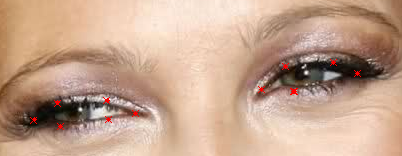
\includegraphics[width=\linewidth]{dissertation//figures/noisy-frame-hrnet.png}
        \caption{HRNet's landmarks on an original image (dots) and perturbed image (crosses)}
    \end{subfigure}
    \begin{subfigure}{0.45\linewidth}
        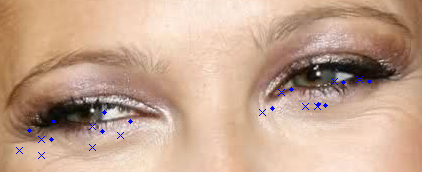
\includegraphics[width=\linewidth]{dissertation//figures/noisy-frame-pfld.png}
        \caption{PFLD's landmarks on an original image (dots) and perturbed image (crosses)}
    \end{subfigure}
    \caption{A comparison of landmarks on original and perturbed images}
    \label{fig:landmarks-noise}
\end{figure}

Both PFLD and HRNet were shown to be resistant to attacks. As such, it is shown that the overall concept of blink-based DeepFake detection is resistant to adversarial noise, rather than just a specific facial landmarking model. This allows for more accurate landmark detectors to be introduced which will produce more accurate EAR graphs which can further improve the accuracy of blink-based detection. 

Overall, blink-based is resistant to adversarial noise attacks because it deals with the abstraction of a video over time. Whilst CNNs classify a video on a per-frame basis, blink detection takes every frame into account. Whilst adversarial noise does affect the exact coordinates of landmarks in some models, as shown in Figure \ref{fig:landmarks-noise}, the added variation in landmarks only makes the resulting EAR graph more varied, highlighting the originating video as a likely fake.

As a result, to produce a successful attack against a blink-based detection model, the noise would need to be consistent across frames to cause a constant mislocation of eye landmarks, to produce an EAR graph that would be classified as real. Such a challenge would require an attack that it is temporally aware. As discussed in Section \ref{sec:blink-based-detection}, neural networks struggle with any problem of a temporal nature, as such noise required to attack a blink-based DeepFake detector would be computationally challenging to produce.

\subsection{Perturbed Traditional Detection}

On the other hand, traditional CNN-based detectors fall significantly in accuracy when exposed to adversarial noise attacks, even when the noise is indirectly attacking the model. As expected, when attacked by adversarial noise, a traditional classifier's accuracy would fall significantly, often to 0\% when attacked with the strongest amount of noise. On average, when opposed to the weak noise ($\epsilon=0.05)$, accuracy decreased to an average of 0.025\%. Similarly, when exposed to higher levels of noise ($\epsilon=0.1$), accuracy on the targeted model would reduce to 0\%; apart from the ResNet model on the Celeb-DF dataset which attained an accuracy of 68.1\%. Whilst still a far cry from the unperturbed accuracy of 99.4\%, it is nonetheless surprising. The experiment was rerun, but the result stayed the same. The results show that lower-strength noise is sufficient to produce a successful attack. FGSM is a black box attack, only needing the input and output of a model, so can be applied to any DeepFake detector that uses a conventional CNN as the backbone.

Furthermore, an FGSM attack is shown to be a general attack. Whilst not as effective as the model being targeted, other models experienced a significant drop in accuracy. VGG was the most vulnerable of the models, dropping to accuracies below 20\% in every scenario and in most cases dropping to below 5\%. On the other hand, Xception proved relatively resilient to indirect adversarial attacks, repeatedly scoring higher than all other indirectly attacked models.

There was a significant variety in accuracy between datasets. EfficientNet would attain high accuracies of 30-60\% on FaceForensics but would drop to under 10\% for Celeb-DF. On the contrary, Xception obtained around 30\% on FaceForensics but would score over 70\% on Celeb-DF when indirectly attacked. This is due to the differences between the two datasets. As stated in Section \ref{sec:un-trad-detect}, Celeb-DF is a more difficult dataset than FaceForensics, hence it contains different DeepFake methods. Therefore, the attacks on each model will be different across datasets as each model will be focusing on different aspects of the image. The resulting noisy images will be different and thus cause different levels of errors on models.

Overall, every traditional model experienced a loss in accuracy when attacked by adversarial noise, either directly or indirectly. This shows that blink-based DeepFake is indeed resilient against adversarial noise as it was not affected by indirect attacks. 

\section{Transferability}

Appendix \ref{sec:transfer} shows the raw results of transferability.

Unfortunately, the results for transferability are inconclusive. There is no correlation between any of the blink-based DeepFake detectors. Whilst they are slightly more accurate than the traditional detectors, none achieve sufficient accuracy across both and real fake videos to be deemed suitable for a general DeepFake detector. Whilst the HRNet model trained on Celeb-DF has a high accuracy score on faked videos (99.7\%), it consistently declares any video as fake, resulting in it having an accuracy of 0.6\% on real videos from the FakeAVCeleb dataset. The accuracies of the other blink detection models bear little similarity with the models they were trained on, meaning they cannot be used as general detectors.

One potential reason for the discrepancy is that whilst real blinking is consistent across datasets, fake blinking is not. One DeepFake may blink too frequently, another may blink for too long, etc. Similar to how a CNN picks up on the irregularities in the data it was trained, so does the time series classifier. The time series classifiers employed in this project have all overfitted on the methods they were trained on and thus cannot be used as general detectors.

As has been shown in literature\cite{ricker2022towards}, CNNs are only effective on the data they are trained on. The same phenomenon is shown in this project. One discovery that is novel to Ricker et al's research is that the models trained for this project seem to consistently classify unknown videos as real. One potential reason is the set threshold for classification. This project uses the most probable class as the final classification, resulting in a threshold of 50\% for classification. If a CNN is unsure of classification, the probability for each class will be close to 50. The CNNs trained in this project have a slight leniency towards a real classification with the average confidence that a frame was real being 52\%, hence a tendency to classify unknown videos as real.

\section{Evaluating Blink-Based DeepFake Detection}

% \begin{itemize}
%     \item mention potential downsides of blink based
%     \begin{itemize}
%         \item required eyes to be constantly visible for reliable detection
%         \item requires eyes to be faked
%     \end{itemize}
%     \item obviously other adversarial noise methods need to be evaluated but ran out of time :(
% \end{itemize}

As shown, the primary benefit of blink-based DeepFake is the native resiliency to adversarial noise attacks. Adversarial Noise is a relatively computationally cheap and reliable way of causing an otherwise accurate DeepFake detector to classify fake videos. Blink-based detectors are resistant to such attacks and therefore can be used reliably when there is suspicion that an image or video has been manipulated. Whilst the accuracy of the detectors produced in this project are relatively inaccurate, they maintain a consistent accuracy above 50\%. As such, they are not merely guessing but making consistent classifications. Therefore, the resiliency to adversarial noise shown is native to the network architecture. If the overall accuracy was to increase to a valid rate (for example, 90\%), then the accuracy on perturbed videos would equally rise. Hence, this project can be used as a proof-of-concept that blink-based DeepFake detection is resistant to adversarial noise and future works can improve on the overall accuracy.

The primary downside to blink-based detection as an architecture is that it requires a video where the subject's eyes are clearly visible throughout the majroity of the runtime. Whilst it is possible to detect landmarks through occlusions, it is significantly less accurate than if the eyes were clearly visible, potentially leading to a misclassification. Furthermore, the eyes need to be faked to be classified. If just the mouth is faked, then blink detection will be unable to classify the video correctly.

Hence, it is recommended that a blink-based DeepFake detector should not be used on its own as a classifier. It should instead be used in two scenarios as a supplement to other detection methods. The first scenario for its use is if a video is suspected to have been attacked with adversarial noise. If a traditional detector is consistently classifying a video as real but something feels ``off" about the video then it is recommended to pass the video through a blink detector for some clarification. 

Another potential use for these detectors is as part of an ensemble of classifiers. Ensemble classifiers are group of classifiers all running on the same video, with the final classification being the majority vote of the classifiers. A blink based detector has a place among the ensemble as a form of resiliency against adversarial noise.